\documentclass[8pt, a4paper, landscape, includeheadfoot]{extarticle}

% Verwendete Pakete

	\usepackage[utf8]{inputenc}
	\usepackage[top=0.2cm, 
	            bottom=0.01cm, 
	            left=0.5 cm, 
	            right=0.5 cm, 
	            footskip = 2.9pt]{geometry}
	\usepackage{babel} % set language to new german
	\usepackage{amsmath}
	\usepackage{amsfonts}
	\usepackage{lmodern}
	\usepackage{graphicx}
	\setlength{\parindent}{0pt}
	\usepackage{ulem} %option rausgenommen
	\usepackage[dvipsnames]{xcolor}%option "table" raus
	\usepackage{enumitem}
	\usepackage{mathabx}
	\usepackage{enumitem}
	\usepackage{colortbl}
	\usepackage{mathtools}
	\usepackage{wallpaper}
	\usepackage{changepage}
	\usepackage{tikz}
	\usepackage{tabularx}
	\usepackage[skins]{tcolorbox}
	\usepackage{lipsum}
	\usepackage{multicol}
	\usepackage{multirow}
	\usepackage{letltxmacro}
	\usepackage{tabularx}
	\usepackage{float}
    \usepackage{amssymb, physics}
    \usepackage{empheq}
    \usepackage{textcomp} % gensymb dependency
    \usepackage{calc} % Multiplikation mit werten ermöglichen
    \usepackage[makeroom]{cancel} %Terme durchstreichen
    \usepackage{mathtools}
    \usepackage{sidecap} %für Bild und Text nebeneinander
    %\usepackage{gensymb} % Degree celcius symbol
    \usepackage{fancyhdr} % Kopfzeile
    \usepackage{romannum} % roman numbers
	\usepackage{makecell} % zeilenumbruch in tabellen


% Spalteneinstellungen

\setlength\columnsep{5mm}
\setlength{\columnseprule}{0.5pt}

%FBOX Einstellungen

\setlength{\fboxrule}{0.5pt}

%Kopf und Fusszeile 

\setlength{\headsep}{0.5em}
\setlength{\footskip}{2.9pt}

\pagestyle{fancy}
\fancyhf{}
\lhead{\textbf{\Subject}}
\chead{Page \thepage{}}
\rhead{\CustomAuthor}
\cfoot{}

% Farbe

\def \customColor {PineGreen}

% Bullet-Symbol für Aufzählungen
\renewcommand\textbullet{\ensuremath{\bullet}}

% Eingekreiste Nummern für Aufzählungen
\newcommand*\circled[1]{\tikz[baseline=(char.base)]{
        \node[shape=circle,draw,inner sep=1.2pt] (char) {#1};}}

% Schriftart
\renewcommand{\familydefault}{\sfdefault}

%Tabelle Horiz. Grösse
\renewcommand{\arraystretch}{1.5}

%Einheiten
\newcommand{\Einheit}[1]{
$\bigl[ #1 \bigr]$
}

\newcommand{\EinheitBruch}[2]{
$\bigl[ \frac{#1}{#2} \bigr]$
}

\newcommand{\Umbruch}{\vfill\null\columnbreak}

% Titel-Block	
\newcommand{\Header}[3]{
	\begin{tcolorbox}  [arc = 0mm, 
	                    colback = \customColor!50!black, 
	                    colframe = \customColor!50!black, 
	                    valign = center, 
	                    fontupper=\color{white}]
		\large \center \textbf{#1} \par
		\huge \textbf{#2} \par 
		\vskip 5pt 
		\large #3 \par
		\vskip 3pt 
		\small Version: \today
	\end{tcolorbox}
	}

%Teil-Block
\newcommand{\Abschnitt}[1]{
	\begin{tcolorbox} [arc = 0mm,
						colback = \customColor!50!black,
						colframe = \customColor,
						valign = center,
						before skip = 3mm,
						leftright skip = -0.5mm,
						after skip = 1 mm,
						bottomrule = 0 mm,
						toprule = 0 mm,
						leftrule = 0 mm,
						rightrule = 0 mm,
						fontupper=\color{white}
						]
		\centering\Large\textbf{#1}
	\end{tcolorbox}
}

% Überschrift
\renewcommand{\section}[1]{
	\begin{tcolorbox}[
			arc=0mm,
			colback=\customColor!50!black,
			colframe=white,
			bottomrule = 0 mm,
			toprule = 0 mm,
			leftrule = 0 mm,
			rightrule = 0 mm,
			valign=center,
			left=0.5mm,
			top= 0.7 mm,
			bottom= 0.7 mm,
			fontupper=\color{white},
			before skip = 1mm,
			leftright skip = -0.5mm,
			after skip = 1 mm]

		\textbf{#1}
	\end{tcolorbox}
	}

% Abschnitt	
\renewcommand{\subsection}[1]{
\begin{tcolorbox}[
            		arc=0mm,
            		colback=\customColor!50,
            		colframe=white,
            		bottomrule = 0 mm,
            		toprule = 0 mm,
            		leftrule = 0 mm,
            		rightrule = 0 mm,
            		valign=center,
            		left=0.5mm,
            		top=0.2mm,
            		bottom=0.2mm,
            		before skip = 1mm,
            		leftright skip = -0.5mm,
            		after skip = 1mm]
	\small \textbf{#1}
\end{tcolorbox}
}

\renewcommand{\subsubsection}[2]{
\begin{tcolorbox}[
            		arc=0mm,
            		colback=gray!50,
            		colframe=white,
            		bottomrule = 0 mm,
            		toprule = 0 mm,
            		leftrule = 0 mm,
            		rightrule = 0 mm,
            		valign=center,
            		left=0.5mm,
            		top=0.2mm,
            		bottom=0.2mm,
            		before skip = 1mm,
            		leftright skip = -0.5mm,
            		after skip = 1mm]
	\small #1 \hfill #2
\end{tcolorbox}
}

%MATH-BOX, optional commands in {}
\newtcbox{\mathbox}[1][]{%
    nobeforeafter, 
    tcbox raise base, 
    colframe=blue!30!black,
    colback=blue!20, 
    boxrule=1pt,
    arc=1mm,
    before skip = 0mm,
    right = 1mm,
    left=1mm,
	top=0.5mm,
	bottom=0.5mm,
    #1}
    
\newtcbox{\mathboxnoback}[1][]{%
    nobeforeafter, 
    tcbox raise base, 
    colframe=black,
    colback=white,
    boxrule=1pt,
    arc=1mm,
    before skip = 0mm,
    right = 1mm,
    left=1mm,
	top=0.5mm,
	bottom=0.5mm,
    #1}
    
\newcommand{\textbox}[1]{
\tcbox[
		arc=1mm,
		colback=blue!20,
		colframe=blue!30!black,
		arc=1mm,
		boxrule=1pt,
		right = 1mm,
        left=1mm,
	    top=0.5mm,
	    bottom=0.5mm,
		before skip = 1mm,
		after skip = 2 mm
		]
{    
	#1
}
}

\newcommand{\textboxmithead}[2]{
\begin{tcolorbox}[
		arc=1mm,
		colback=blue!20,
		colframe=blue!30!black,
		arc=1mm,
		boxrule=1pt,
		left=1mm,
		top= 1 mm,
		bottom= 1 mm,
		before skip = 2mm,
		leftright skip = 8mm,
		after skip = 2 mm
		]
    \centering{\textbf{#1}\par}
	#2
\end{tcolorbox}
}

\newtcolorbox{titlebox}[1][]{
        fonttitle=\bfseries, 
        colbacktitle=gray!80,
        enhanced,
        attach boxed title to top center={yshift=-2mm},
        colframe=black,
        colback=white,
        boxrule=1pt,
        arc=1mm,
        before skip = 2mm,
        right = 1mm,
        left=1mm,
    	top=0.5mm,
    	bottom=0.5mm,
        title=#1}



\def \Subject {CS229 - Machine Learning}
\def \CustomTitle {Linear Algebra \& Probability}
\def \CustomAuthor {Tim Reinhart - rtim@stanford.edu}

\begin{document}
\pagenumbering{arabic}
\begin{multicols*}{4}
	\Header{\Subject}{\CustomTitle}{\CustomAuthor}

	\section{Matrices}

	\subsection{Matrix Multiplication}

	Matrices can be multiplied with each other in the following manner:

	\begin{center}
		\fbox{
			$A \cdot B = C \hspace{5pt} \Rightarrow \hspace{5pt} c_{ik} = \sum_{j=1}^n a_{ij} \cdot b_{jk}$
		}
	\end{center}

	\begin{center}
		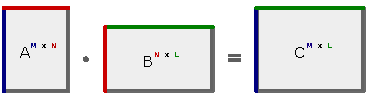
\includegraphics[width = 0.95 \columnwidth]{0_images/Matrixmultiplikation.pdf}
	\end{center}

	\textbf{Associative \& Distributive Laws:}

	\begin{center}
		\parskip3pt
		\begin{align}
			(A\cdot B) \cdot C & = A \cdot (B \cdot C) \nonumber   \\
			(A + B) \cdot C    & = A \cdot C + B \cdot C \nonumber \\
			A \cdot (C + D)    & = A \cdot C + A \cdot D \nonumber
		\end{align}
	\end{center}
	\textbf{Warning!} The commutative law does not apply! Generally, $A\cdot B \neq B \cdot A$.

	\subsection{Transpose}

	The transpose of a matrix is obtained by "mirroring" it along its diagonal.

	\begin{center}
		\textbf{Example:}
		$\begin{pmatrix}
				a & b \\
				c & d \\
				e & f \\
			\end{pmatrix}^T
			=
			\begin{pmatrix}
				a & c & e \\
				b & d & f \\
			\end{pmatrix}$
	\end{center}

	\textbf{Calculation Rules:}

	\vspace{-5mm}
	\begin{minipage}[t]{0.49 \columnwidth}
		\begin{align}
			(A + B)^T     & = A^T + B^T \nonumber     \\
			(A \cdot B)^T & = B^T \cdot A^T \nonumber \\
			(c \cdot A)^T & = c \cdot A^T \nonumber   \\
			(A^T)^T       & = A \nonumber
		\end{align}
	\end{minipage}
	\begin{minipage}[t]{0.49 \columnwidth}
		\begin{align}
			(A^T)^{-1} & = (A^{-1})^T \nonumber \\
			rank(A^T)  & = rank(A) \nonumber    \\
			det(A^T)   & = det(A) \nonumber     \\
			eig(A^T)   & = eig(A) \nonumber
		\end{align}
	\end{minipage}


	\subsection{Inverse}

	The inverse \( A^{-1} \) of \( A \) reverses a multiplication with \( A \). When you multiply \( A \) with \( A^{-1} \), you get the identity matrix.

	\textbf{Properties:}

	\begin{itemize}[leftmargin=0.29cm, itemsep=0pt]
		\item Only square matrices can be invertible.
		\item An invertible matrix is called \textbf{regular}, a non-invertible one \textbf{singular}.
		\item The inverse is unique.
		\item \( A \) is invertible if and only if \( A \) has full rank.
		\item \( A \) is invertible if and only if \( A^T \) is invertible.
		\item \( A \) is symmetric if and only if \( A^{-1} \) is symmetric.
		\item \( A \) is a triangular matrix if and only if \( A^{-1} \) is a triangular matrix.
		\item \( A \) is invertible if and only if \( \text{det}(A) \neq 0 \).
		\item \( A \) is invertible if and only if no eigenvalue \( \lambda = 0 \).
		\item \( A \) and \( B \) are invertible implies \( AB \) is invertible.
	\end{itemize}

	\textbf{Calculation rules:}

	\vspace{-5mm}
	\begin{minipage}[t]{0.49 \columnwidth}
		\begin{align}
			I^{-1}          & = I\nonumber                    \\
			(A^{-1})^{-1}   & = A \nonumber                   \\
			(A^k)^{-1}      & = (A^{-1})^k \nonumber          \\
			(c\cdot A)^{-1} & = c^{-1} \cdot A^{-1} \nonumber \\
			(A\cdot B)^{-1} & = B^{-1} \cdot A^{-1} \nonumber
		\end{align}
	\end{minipage}
	\begin{minipage}[t]{0.49 \columnwidth}
		\begin{align}
			(A^T)^{-1}   & = (A^{-1})^T \nonumber  \\
			rang(A^{-1}) & = rang(A) \nonumber     \\
			det(A^{-1})  & = det(A)^{-1} \nonumber \\
			eig(A^{-1}   & = eig(A)^{-1} \nonumber
		\end{align}
	\end{minipage}

	\subsection{Matrix Tricks}

	\textbf{Probability Rules for Matrices:}

	• Pull Matrix Multiply out of Variance:
	$$
		Var[Mx] = MVar[x]M^T
	$$

	\subsection{Eigenvalues and Eigenvectors}

	\begin{empheq}[box = \mathboxnoback]{align*}
		\text{Eigenvalues of A: } \det(A - \lambda\cdot I) = 0
	\end{empheq}

	\textbf{Verify Computation}

	\begin{itemize}[leftmargin=0.29cm, itemsep=0.5pt]
		\item Trace(A) = \( a_{11} + a_{22} + \dots + a_{nn} = \sum \lambda_i \)
		\item det(A) = product of \( \lambda_i \)
	\end{itemize}

	\textbf{Eigenvectors: } Kernel of the matrix $A - \lambda_i\cdot I$, where \( \lambda_i \) is the eigenvalue corresponding to the eigenvector.

	\subsection{Determinant}

	\textbf{Block Sentence for Determinant Computation}

	\begin{center}
		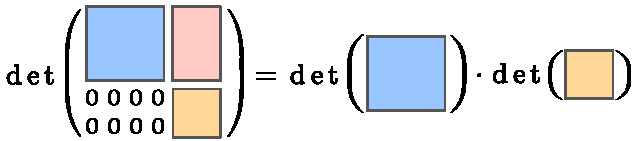
\includegraphics[width = 0.8 \columnwidth]{0_images/Blocksatz.pdf}
	\end{center}

	\subsection{Positive (Semi-)Definite Matrices}
	\subsubsection{Definitions}{}
	A symmetric matrix \( A \in \mathbb{R}^{n \times n} \) is called:
	\begin{itemize}[itemsep=0pt]
		\item \textbf{Positive Semi-Definite (PSD)} if for any non-zero vector \( \mathbf{x} \in \mathbb{R}^n \), we have \( \mathbf{x}^T A \mathbf{x} \geq 0 \).
		\item \textbf{Positive Definite (PD)} if for any non-zero vector \( \mathbf{x} \in \mathbb{R}^n \), \( \mathbf{x}^T A \mathbf{x} > 0 \).
	\end{itemize}

	\subsubsection{Properties}{}
	\begin{itemize}[itemsep=0pt]
		\item All eigenvalues of a PSD matrix are non-negative, and those of a PD matrix are positive.
		\item A matrix is PSD if and only if it can be written as \( B^T B \), where \( B \) is any matrix.
		\item If \( A \) is PD (or PSD), then so is \( A^{-1} \) (if \( A \) is invertible).
		\item For any matrix \( A \), the matrices \( A^T A \) and \( AA^T \) are PSD.
		\item The sum of two PSD matrices is also PSD.
	\end{itemize}

	\subsubsection{Checking for Positive (Semi-) Definiteness}{}
	Determining if a matrix is PSD or PD can be done in several ways:

	\begin{itemize}[itemsep=0pt]
		\item \textbf{Eigenvalue Criterion:} A symmetric matrix is PSD if and only if all its eigenvalues are non-negative. It is PD if all eigenvalues are positive.
		\item \textbf{Principal Minors:} A symmetric matrix \( A \) is PD if all its leading principal minors (determinants of the top-left \( k \times k \) submatrix, \( 1 \leq k \leq n \)) are positive. For PSD, all leading principal minors should be non-negative.
		\item \textbf{Cholesky Decomposition:} A matrix is PD if and only if it has a Cholesky decomposition. For numerical algorithms, attempting a Cholesky decomposition and checking for failure can be an effective way to test for positive definiteness.
	\end{itemize}

	\section{Matrix Calculus}
	\subsection{Gradient}
	The gradient of a scalar function $f: \mathbb{R}^n \rightarrow \mathbb{R}$ with respect to a vector $\mathbf{x} \in \mathbb{R}^n$ is a vector of partial derivatives:
	$$
		\nabla f(\mathbf{x}) = \begin{pmatrix}
			\frac{\partial f}{\partial x_1} \\
			\frac{\partial f}{\partial x_2} \\
			\vdots                          \\
			\frac{\partial f}{\partial x_n}
		\end{pmatrix}
	$$

	\subsection{Hessian}
	The Hessian matrix of a scalar-valued function $f: \mathbb{R}^n \rightarrow \mathbb{R}$ is a square matrix of second-order partial derivatives:
	$$
		H(f)(\mathbf{x}) = \begin{pmatrix}
			\frac{\partial^2 f}{\partial x_1^2}            & \frac{\partial^2 f}{\partial x_1 \partial x_2} & \cdots & \frac{\partial^2 f}{\partial x_1 \partial x_n} \\
			\frac{\partial^2 f}{\partial x_2 \partial x_1} & \frac{\partial^2 f}{\partial x_2^2}            & \cdots & \frac{\partial^2 f}{\partial x_2 \partial x_n} \\
			\vdots                                         & \vdots                                         & \ddots & \vdots                                         \\
			\frac{\partial^2 f}{\partial x_n \partial x_1} & \frac{\partial^2 f}{\partial x_n \partial x_2} & \cdots & \frac{\partial^2 f}{\partial x_n^2}
		\end{pmatrix}
	$$

	\subsection{Examples}

	\subsubsection{\( f(\mathbf{x}) = \mathbf{A}\mathbf{x} \)\hfill $\mathbf{A}\in\mathbb{R}^{m\times n}$}{}

	Gradient:
	$$
		\nabla_x f = \mathbf{A}^T
	$$

	\subsubsection{\( f(\mathbf{x}) = \mathbf{x}^T\mathbf{A}\mathbf{x} \)\hfill $\mathbf{A}\in\mathbb{R}^{m\times n}$}{}

	Gradient:
	$$
		\nabla_x f = (\mathbf{A} + \mathbf{A}^T)\mathbf{x} = 2\mathbf{Ax} \quad \text{ if sym.}
	$$

	Hessian:
	$$
		H(f) = \mathbf{A} + \mathbf{A}^T = 2\mathbf{A}\quad \text{ if sym.}
	$$

	\subsubsection{Linear Regression Loss (\( \ell_2 \) \textbf{norm})}{}
	For the loss function \( L(\mathbf{w}) = ||\mathbf{y} - \mathbf{X}\mathbf{w}||^2 \):

	Gradient:
	$$
		\nabla L = -2\mathbf{X}^T(\mathbf{y} - \mathbf{X}\mathbf{w})
	$$

	Hessian:
	$$
		H(L) = 2\mathbf{X}^T\mathbf{X}
	$$


	\subsubsection{Logistic Regression Loss}{}

	\begin{itemize}
		\item Binary classification with labels \( y_i \in \{0, 1\} \)
		\item Predicted probabilities \( p_i = \frac{1}{1 + e^{-\mathbf{x}_i^T \mathbf{w}}} \)
		\item \( L(\mathbf{w}) = -\sum_{i}[y_i \log(p_i) + (1-y_i) \log(1 - p_i)] \)
	\end{itemize}

	Gradient:
	$$
		\nabla L = \mathbf{X}^T(\mathbf{p} - \mathbf{y})
	$$

	Hessian:
	$$
		H(L) = \mathbf{X}^T \mathbf{S} \mathbf{X}
	$$

	where \( \mathbf{S} \) is a diagonal matrix with \( S_{ii} = p_i (1 - p_i) \).


	\section{Basic Probability}
	\subsection{Bayes Theorem}

	$$
		P(X{=}x | Y{=}y) = \frac{P(Y{=}y | X{=}x) P(X{=}x)}{P(Y{=}y)}
	$$

	Where:
	\begin{itemize}
		\item $P(X{=}x | Y{=}y)$ is the posterior probability: the probability of event $X{=}x$ given that $Y{=}y$ has occurred.
		\item $P(Y{=}y | X{=}x)$ is the likelihood: the probability of observing $Y{=}y$ given $X{=}x$.
		\item $P(X{=}x)$ is the prior probability: the initial belief about $X{=}x$.
		\item $P(Y{=}y)$ is the marginal probability: the total probability of observing $Y{=}y$ under all possible outcomes of $X$.
	\end{itemize}
	\subsubsection{Law of Total Probability}

	A key concept related to Bayes' Theorem is the Law of Total Probability. It is useful for calculating $P(Y{=}y)$, the marginal probability in Bayes' formula, especially when dealing with compound events. The law states:

	$$
		P(Y{=}y) = \sum_{i} P(Y{=}y | X{=}x_i) P(X{=}x_i)
	$$

	Where $X{=}x_i$ represents all disjoint outcomes that cover the sample space. In the context of Bayes' Theorem, it's used to marginalize over the different possible states of knowledge or evidence.

	\subsubsection{Bayes' Rule for Multiple Events}

	In cases involving more than two events, Bayes' Theorem can be generalized as:
	\begin{align*}
		 & P(X_1{=}x_1, \ldots, X_n{=}x_n | Y{=}y)                                                \\
		 & = \frac{P(Y{=}y | X_1{=}x_1, \ldots, X_n{=}x_n)\prod_{i=1}^{n} P(X_n{=}x_n)}{P(Y{=}y)}
	\end{align*}

	\subsubsection{Bayes' Theorem with Continuous Variables}

	When dealing with continuous variables, Bayes' Theorem takes the form of probability densities:

	$$
		f_{X|Y}(x|y) = \frac{f_{Y|X}(y|x) f_X(x)}{f_Y(y)}
	$$

	Where $f_{X|Y}(x|y)$ is the conditional density of $X$ given $Y$, and so on.

	\subsubsection{Prior and Posterior Probabilities}

	In Bayesian analysis, the prior probability $P(X{=}x)$ represents our belief about $X$ before observing the evidence $Y$, while the posterior probability $P(X{=}x | Y{=}y)$ is our updated belief after observing $Y$. The transformation from the prior to the posterior, via the likelihood and marginal likelihood, is the essence of Bayesian inference.

	\subsection{Expectation Value}

	\begin{align*}
		 & \operatorname{E}[X] = \sum_i x_i p_i \quad \text{(for discrete var.)} \quad \text{or}                                        \\
		 & \operatorname{E}[X] \equiv \int_\Omega X \, d\operatorname{P} = \int_{\mathbb{R}} x f(x) \, dx \quad \text{(for cont. var.)}
	\end{align*}

	\subsubsection{Properties of Expectation}{}

	\paragraph{Linearity}
	The expectation operator is linear:
	$$
		\operatorname{E}[aX + bY] = a\operatorname{E}[X] + b\operatorname{E}[Y]
	$$
	where \(a\) and \(b\) are constants, and \(X\) and \(Y\) are random variables.

	\paragraph{Monotonicity}
	If \(X \leq Y\) (i.e., \(X\) is always less than or equal to \(Y\)), then:
	$$
		\operatorname{E}[X] \leq \operatorname{E}[Y]
	$$

	\paragraph{Law of the Unconscious Statistician}
	This law states that if \(Y = g(X)\) for some function \(g\), then:
	$$
		\operatorname{E}[Y] = \operatorname{E}[g(X)] = \sum_x g(x) P(X = x) \quad \text{(discrete case)}
	$$
	or
	$$
		\operatorname{E}[g(X)] = \int_{-\infty}^{+\infty} g(x) f_X(x) \, dx \quad \text{(continuous case)}
	$$
	where \(f_X(x)\) is the probability density function of \(X\).

	\paragraph{Independence}
	If two random variables \(X\) and \(Y\) are independent, then:
	$$
		\operatorname{E}[XY] = \operatorname{E}[X] \cdot \operatorname{E}[Y]
	$$

	\subsubsection{Conditional Expectation}{}

	\begin{align*}
		\operatorname{E}(X | Y = y) & =  \sum_x x P(X = x | Y = y)                \\
		                            & = \sum_x x \frac{P(X = x, Y = y)}{P(Y = y)}
	\end{align*}

	\subsection{Variance}

	Variance quantifies the spread or dispersion of a set of data points or the spread of a probability distribution. It is defined as the expected value of the squared deviation from the mean (denoted by \(\mu\)):

	\begin{align*}
		Var(X) = \operatorname{E}[\left(X - \mu\right)^2] = \operatorname{E}[X^2] - (\operatorname{E}[X])^2
	\end{align*}

	\subsubsection{Properties of Variance}

	\paragraph{Non-negativity}
	The variance is always non-negative:
	$$
		Var(X) \geq 0
	$$

	\paragraph{Variance of a Constant}
	$$
		Var(a) = 0
	$$
	where \(a\in\mathbb{R}\) is a constant.

	\paragraph{Factor Out Constants}
	$$
		Var(aX) = a^2 Var(X)
	$$
	where \(a\in\mathbb{R}\) is a constant.

	\paragraph{Variance of a Sum}
	For any random variables \(X\), \(Y\):
	\begin{align*}
		\operatorname{Var}(aX + bY) & =a^2\operatorname{Var}(X)+b^2\operatorname{Var}(Y) \\
		                            & +2ab\, \operatorname{Cov}(X,Y)                     \\
		\operatorname{Var}(aX - bY) & =a^2\operatorname{Var}(X)+b^2\operatorname{Var}(Y) \\
		                            & -2ab\, \operatorname{Cov}(X,Y)
	\end{align*}
	If \(X\) and \(Y\) are independent, then \(Cov(X, Y) = 0\), and this simplifies to:
	$$
		\operatorname{Var}(aX \pm bY) =a^2\operatorname{Var}(X)+b^2\operatorname{Var}(Y)
	$$

	\paragraph{Sum of uncorrelated variables}

	\begin{align*}
		\operatorname{Var}\left(\sum_{i=1}^n X_i\right) = \sum_{i=1}^n \operatorname{Var}(X_i)
	\end{align*}

	\paragraph{Sum of correlated variables}
	\begin{align*}
		\operatorname{Var}\left(\sum_{i=1}^n X_i\right) & = \sum_{i=1}^n \sum_{j=1}^n \operatorname{Cov}\left(X_i, X_j\right)                                                                    \\
		                                                & = \sum_{i=1}^n \operatorname{Var}\left(X_i\right) + 2\hskip-10pt\sum_{1\le i<j\le n}\hskip-10pt\operatorname{Cov}\left(X_i, X_j\right)
	\end{align*}

	\section{Probability Distributions}

	\subsection{Discrete Distributions}

	\subsubsection{Bernoulli Distribution}{}
	One Trial, Two outcomes
	\paragraph{PMF:}
	\begin{align*}
		P(y;\phi) = \begin{cases}
			\phi     & y = 1 \\
			1 - \phi & y = 0
		\end{cases} \\
		P(y;\phi) = \phi^y (1-\phi)^{1-y} \quad \text{for } y \in \{0,1\}
	\end{align*}

	\paragraph{Mean and Variance:}
	$$
		\mu = p, \quad \sigma^2 = p(1 - p)
	$$

	\subsubsection{Binomial Distribution}{}
	Distribution of the number of successes in a sequence of $n$ independent experiments, each with two outcomes, and each with its own Boolean-valued outcome: success (with probability $p$) or failure (with probability $q = 1 -p$)
	$\rightarrow$ Multiple Trials, Two outcomes
	\paragraph{PMF:}
	The probability of getting exactly $k$ successes in $n$ independent Bernoulli trials (with the same rate $p$) is given by
	$$
		P(X = k) = \binom{n}{k} p^k (1-p)^{n-k}
	$$
	\paragraph{Mean and Variance:}
	$$
		\mu = np, \quad \sigma^2 = np(1 - p)
	$$

	\subsubsection{Multinomial Distribution}{}
	Multiple Trials, Multiple outcomes
	\paragraph{PMF:}
	$$
		P(\mathbf{X} = \mathbf{x}) = \frac{n!}{x_1! x_2! \cdots x_k!} p_1^{x_1} p_2^{x_2} \cdots p_k^{x_k}
	$$
	\paragraph{Mean and Variance:}
	For each category $i$,
	$$
		\mu_i = np_i, \quad \sigma^2_i = np_i(1 - p_i)
	$$
	Covariance for categories $i$ and $j$,
	$$
		\mathrm{Cov}(X_i, X_j) = -np_i p_j \quad (i \neq j)
	$$

	\subsubsection{Poisson Distribution}{}
	\paragraph{PMF:}
	$$
		P(X = k) = \frac{\lambda^k e^{-\lambda}}{k!}
	$$
	\paragraph{Mean and Variance:}
	$$
		\mu = \sigma^2 = \lambda
	$$

	\subsubsection{Geometric Distribution}{}
	\paragraph{PMF:}
	$$
		P(X = k) = (1-p)^{k-1} p
	$$
	\paragraph{Mean and Variance:}
	$$
		\mu = \frac{1}{p}, \quad \sigma^2 = \frac{1 - p}{p^2}
	$$

	\subsection{Continuous Distributions}

	\subsubsection{Exponential Distribution}{}
	\paragraph{PDF:}
	$$
		f(x) = \lambda e^{-\lambda x}, \quad x \geq 0
	$$
	\paragraph{Mean and Variance:}
	$$
		\mu = \frac{1}{\lambda}, \quad \sigma^2 = \frac{1}{\lambda^2}
	$$

	\subsubsection{Uniform Distribution}{}
	\paragraph{PDF:}
	$$
		f(x) = \frac{1}{b - a} \quad \text{for } a \leq x \leq b
	$$
	\paragraph{Mean and Variance:}
	$$
		\mu = \frac{a + b}{2}, \quad \sigma^2 = \frac{(b - a)^2}{12}
	$$

	\subsubsection{Beta Distribution}{}
	\paragraph{PDF:}
	$$
		f(x; \alpha, \beta) = \frac{x^{\alpha - 1} (1 - x)^{\beta - 1}}{\mathrm{B}(\alpha, \beta)}
	$$
	\paragraph{Mean and Variance:}
	$$
		\mu = \frac{\alpha}{\alpha + \beta}, \quad \sigma^2 = \frac{\alpha \beta}{(\alpha + \beta)^2 (\alpha + \beta + 1)}
	$$

	\subsubsection{Gamma Distribution}{}
	\paragraph{PDF:}
	$$
		f(x; \alpha, \beta) = \frac{\beta^\alpha x^{\alpha - 1} e^{-\beta x}}{\Gamma(\alpha)} \quad \text{for } x > 0
	$$
	\paragraph{Mean and Variance:}
	$$
		\mu = \frac{\alpha}{\beta}, \quad \sigma^2 = \frac{\alpha}{\beta^2}
	$$

	\subsubsection{Dirichlet Distribution}{}
	\paragraph{PDF:}
	$$
		f(\mathbf{x}; \boldsymbol{\alpha}) = \frac{1}{\mathrm{B}(\boldsymbol{\alpha})} \prod_{i=1}^{K} x_i^{\alpha_i - 1}
	$$
	Where $\mathrm{B}(\boldsymbol{\alpha})$ is the multivariate beta function.
	\paragraph{Mean and Variance:}
	For each component $i$,
	$$
		\mu_i = \frac{\alpha_i}{\sum_{j=1}^K \alpha_j}
	$$
	\subsection{Exponential Family}
	A single-parameter exponential family is a set of probability distributions
	whose probability density function (or probability mass function, for the case of a discrete distribution) can be expressed in the form
	$$
		p(y;\eta) = b(\eta)\,\exp\bigl[\,\eta^T \, T(y) - a(\eta)\,\bigr]
	$$
	\begin{itemize}[itemsep=0pt]
		\item $\eta$: natural parameter
		\item $T(y)$: sufficient statistic
		\item $a(\eta)$: log partition function
	\end{itemize}

	\subsubsection{Canonical Response Funtion}{}
	$$
		g(\eta) = \operatorname{E}[T(y);\eta]
	$$
	\begin{itemize}[itemsep=0pt]
		\item For the Gaussian family: identify function
		\item For the Bernoulli family: logistic function
	\end{itemize}

	\section{Gaussian Distributions}
	\subsection{Univariate Gaussian}
	The probability density of a univariate Gaussian distribution is given by:
	$$
		\mathcal{N}(x ; \mu, \sigma^2) = \frac{1}{\sqrt{2\pi \sigma^2}} \exp\left( -\frac{(x-\mu)^2}{2\sigma^2} \right)
	$$
	Where $\mu$ is the mean and $\sigma^2$ is the variance.

	\subsection{Multivariate Gaussian}
	The probability density of a multivariate Gaussian distribution in $d$ dimensions is:

	\vskip5pt

	\resizebox{\hsize}{!}{%
		$
			\mathcal{N}(\mathbf{x} ;\boldsymbol{\mu}, \Sigma) = \frac{1}{\sqrt{(2\pi)^k |\Sigma|}} \exp\left( -\frac{1}{2} (\mathbf{x} - \boldsymbol{\mu})^T \Sigma^{-1} (\mathbf{x} - \boldsymbol{\mu}) \right)
		$
	}
	\vskip5pt

	Where $\boldsymbol{\mu}\in\mathbb{R}^d$ is the mean vector, $\Sigma\in\mathbb{R}^{d\times d}$ is the covariance matrix.

	\subsubsection{Mean Vector and Covariance Matrix}{}
	\begin{itemize}
		\item The mean vector \(\boldsymbol{\mu}\) represents the mean of each dimension. If \(\mathbf{x}\) is an \(n\)-dimensional random vector, then \(\boldsymbol{\mu}\) is given by \(\boldsymbol{\mu} = \operatorname{E}[\mathbf{x}]\).
		\item The covariance matrix \(\Sigma\) is symmetric and positive semi-definite. It represents how each pair of dimensions of the random vector \(\mathbf{x}\) co-varies. If \(\mathbf{x}\) has dimensions \(x_1, x_2, ..., x_n\), then the element \(\Sigma_{ij}\) of the matrix \(\Sigma\) is the covariance between \(x_i\) and \(x_j\): \(\Sigma_{ij} = \operatorname{Cov}(x_i, x_j)\).
		\item The determinant of \(\Sigma\) (denoted as \(|\Sigma|\)) and its inverse \(\Sigma^{-1}\) play a key role in defining the shape and orientation of the multivariate Gaussian distribution in its multi-dimensional space.
	\end{itemize}

	\section{Maximum Likelihood Estimation (MLE)}

	\subsection{Definition}
	The likelihood function for a model parameter \(\theta\) given observations \(X = (x_1, x_2, ..., x_n)\) is defined as:
	\[
		\mathcal{L}(\theta | X) = P(X | \theta) = \prod_{i=1}^{n} P(x_i | \theta)
	\]
	where \(P(x_i | \theta)\) is the probability of observing \(x_i\) given the parameter \(\theta\).

	For Discriminative Algorithms:
	\begin{align*}
		\mathcal{L}(\theta) = \prod_{i=1}^{n} p(y^{(i)}\mid x^{(i)}; \theta)
	\end{align*}

	For Generative Algorithms:
	\begin{align*}
		\mathcal{L}(\theta) = \prod_{i=1}^{n} p(x^{(i)}\mid y^{(i)}; \theta)\cdot p(y^{(i)};\theta)
	\end{align*}
	\subsection{Estimation}
	The MLE \(\hat{\theta}\) is the value of \(\theta\) that maximizes \(\mathcal{L}(\theta | X)\). In practice, it's often more convenient to maximize the log-likelihood because the logarithm is a strictly increasing function and transforms the product into a sum, simplifying the differentiation:
	\[
		\ell(\theta | X) = \log \mathcal{L}(\theta | X) = \sum_{i=1}^{n} \log P(x_i | \theta)
	\]

	\subsection{Finding the MLE}
	To find the MLE, we take the derivative of \(\ell(\theta | X)\) with respect to \(\theta\) and set it to zero (for parameter \(\theta\) where this is possible):
	\[
		\frac{\partial}{\partial \theta} \ell(\theta | X) = 0
	\]
	Solving this equation gives us the MLE \(\hat{\theta}\). In cases where the derivative does not exist or the equation is hard to solve, numerical methods such as gradient descent can be used.

	\subsection{Properties of MLE}
	\begin{itemize}[itemsep=0pt]
		\item \textbf{Consistency:} As the number of observations \(n\) approaches infinity, the MLE converges in probability to the true value of \(\theta\).
		\item \textbf{Asymptotic normality:} Under regular conditions, as \(n\) increases, the distribution of \(\hat{\theta}\) approaches a normal distribution centered around the true \(\theta\), with a variance that can be estimated from the data.
		\item \textbf{Invariance:} If \(\hat{\theta}\) is the MLE of \(\theta\), and \(g\) is a function, then the MLE of \(g(\theta)\) is \(g(\hat{\theta})\).
		\item \textbf{Efficiency:} Under certain conditions, MLE achieves the Cramér-Rao lower bound, making it the most efficient unbiased estimator.
	\end{itemize}

	\subsection{Examples}
	\subsubsection{MLE for Normal Distribution}{}
	Consider a dataset \( X = \{ x_1, x_2, \ldots, x_n \} \) assumed to be drawn from a normal distribution \(\mathcal{N}(\mu, \sigma^2)\). The MLE for \(\mu\) and \(\sigma^2\) are given by:
	\[
		\hat{\mu} = \frac{1}{n} \sum_{i=1}^{n} x_i, \quad \hat{\sigma}^2 = \frac{1}{n} \sum_{i=1}^{n} (x_i - \hat{\mu})^2
	\]

	\subsubsection{MLE for a Binomial Distribution}{}
	For a binomial distribution \(B(n, p)\) with known \(n\) and unknown \(p\), given \(k\) successes in \(n\) trials, the MLE of \(p\) is:
	\[
		\hat{p} = \frac{k}{n}
	\]


	\section{Optimization Methods in Machine Learning}

	\subsection{Newton's Method}
	Given a twice-differentiable function \(f(\mathbf{x})\), Newton's method updates the parameter vector \(\mathbf{x}\) as follows:
	\[
		\mathbf{x}_{\text{new}} = \mathbf{x} - \left[\nabla^2 f(\mathbf{x})\right]^{-1} \nabla f(\mathbf{x})
	\]
	where \(\nabla f(\mathbf{x})\) and \(\nabla^2 f(\mathbf{x})\) are the gradient and Hessian matrix of \(f\) at \(\mathbf{x}\), respectively. Despite its quadratic convergence rate, Newton's method can be computationally expensive due to the need to compute and invert the Hessian matrix.

	\subsection{Stochastic Gradient Descent (SGD)}
	Stochastic Gradient Descent is a simplification of the traditional gradient descent algorithm. It updates the parameters using the gradient of the loss function with respect to a \textbf{single} data point (or a small subset) chosen randomly in each iteration. The update rule is:
	\[
		\mathbf{x}_{\text{new}} = \mathbf{x} - \eta \nabla f_i(\mathbf{x})
	\]
	where \(\eta\) is the learning rate, and \(\nabla f_i(\mathbf{x})\) is the gradient computed for the \(i\)th data point. While SGD can be noisy compared to full-batch gradient descent, it allows for more frequent updates, which can be beneficial for large datasets.

	\subsection{Mini-Batch Gradient Descent}
	Mini-Batch Gradient Descent is a variation of SGD where instead of using a single sample at each iteration, a mini-batch of samples is used. This method aims to balance the efficiency of using batches with the reduced variance of the gradient estimate. The update rule for a mini-batch is:
	\[
		\mathbf{x}_{\text{new}} = \mathbf{x} - \eta \nabla f_{\mathbf{B}}(\mathbf{x})
	\]
	where \(\mathbf{B}\) represents a mini-batch of samples and \(\nabla f_{\mathbf{B}}(\mathbf{x})\) is the gradient of the loss function averaged over all samples in the mini-batch.

	\subsection{Normal Equation for Linear Least Squares}
	The Normal Equation is a method to analytically solve the linear least squares problem for finding the best-fitting parameters in a linear regression model. Given a design matrix \(\mathbf{X}\) and a target vector \(\mathbf{y}\), the optimal parameter vector \(\mathbf{w}\) is given by:
	\[
		\mathbf{w} = \left(\mathbf{X}^\top \mathbf{X}\right)^{-1} \mathbf{X}^\top \mathbf{y}
	\]
	This equation directly computes the parameters that minimize the squared difference between the predictions and the actual values. It's computationally efficient for small to moderate-sized datasets but can be computationally expensive or numerically unstable for very large datasets.

	\section{Important Theorems}

	\subsection{Jensen's Inequality}

	Let $X$ be an integrable real-valued random variable and $\phi$ a convex function. Then:

	$$\varphi\left(\operatorname{E}[X]\right) \leq \operatorname{E} \left[ \varphi(X) \right]$$
	\begin{center}
		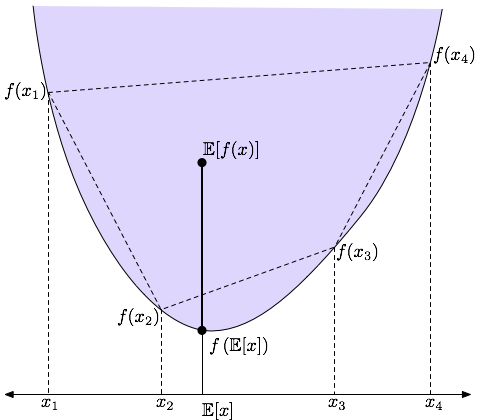
\includegraphics[width=0.8\linewidth]{0_images/jensen.png}
	\end{center}

	\subsection{Concavity}
	A real-valued function $f$	 on an interval (or, more generally, a convex set in vector space) is said to be concave if, for any $x$ and $y$ in the interval and for any $\alpha\in[0,1]$:
	\begin{align*}
		f((1-\alpha )x+\alpha y)\geq (1-\alpha ) f(x)+\alpha f(y)
	\end{align*}

	\section{Decision Trees}
	\subsection{Feature Split selection}
	Given a subset of data $M$ (node in a tree).
	\begin{enumerate}[itemsep=0pt]
		\item For each feature $h_i(x)$:
		      \begin{enumerate}
			      \item Split data of $M$ according to feature $h_i(x)$
			      \item Compute misclassification error of split:
			            \begin{align*}
				            \frac{\# \ \text{mistakes}}{\#\ \text{datapoints}}
			            \end{align*}
		      \end{enumerate}
		\item Choose feature $h^\star$ with lowest error
	\end{enumerate}

	\subsection{Threshold Split Selection}
	\begin{enumerate}[itemsep=0pt]
		\item Sort the values of a feature $h_j(x)$. Let $\{v_1, \dots, v_n\}$ denote sorted values.
		\item For $i = 1\dots n-1$:
		      \begin{enumerate}[itemsep=0pt]
			      \item Consider split $t_i = \frac{v_i + v_[i+1]}{2}$
			      \item Compute error for split $h_j(x)\geq t_i$
		      \end{enumerate}
		\item Choose $t^\star$ with lowest error
	\end{enumerate}
	Threshold split caveat: same feature can be used multiple times!

	\subsection{Greedy Decision Tree Learning}
	\begin{enumerate}[itemsep=0pt]
		\item Start with empty tree
		\item Select a feature to split on (see above)
		\item For each split of tree:
		      \begin{enumerate}[itemsep=0pt]
			      \item If done, make predictions $\rightarrow$ Stopping Cond.
			      \item Otherwise, go to step 2 and recurse on this split
		      \end{enumerate}
	\end{enumerate}

	\subsubsection{Stopping Conditions}{}
	\begin{itemize}[itemsep=0pt]
		\item All data agrees on $y$
		\item Already split on all features
		\item NOT: Error does not decrease!
	\end{itemize}

	\subsection{Tree Pruning Algorithm}
	Repeat for every split in Tree:
	\begin{enumerate}[itemsep=0pt]
		\item Compute total cost $C(T)$ of split using nr. of leaves $L(T)$:
		      \begin{align*}
			      C(T) = \text{Error}(T) + \lambda L(T)
		      \end{align*}
		\item Undo the split to get $T_{small}$ and calculate cost of smaller tree
		\item Prune split if total cost is lower
	\end{enumerate}
	\section{Boosting}
	Classification $y = \pm 1$ from input $x$. Ensemble model consists of classifiers $f_1(x), \dots, f_T(x)$ and coefficients $\hat{w}_1, \dots, \hat{w}_T$. Prediciton:
	\begin{align}
		\hat{y} = sign\left(\sum \hat{w}_t f_t(x)\right)
	\end{align}
	Boosting: focus learning on 'hard' points, using weighted data. Each $x_i, y_i$ weighted by $\alpha_i$. Loss function becomes:
	\begin{align*}
		\sum_{i=1}^{n}\alpha_i\ell(x_i, y_i; \theta)
	\end{align*}
	Gradient of loss will be multiplied by $\alpha_i$, in a decision tree a data point counts $\alpha_i$ times.
	\subsection{AdaBoost Algorithm}
	\begin{enumerate}[itemsep=0pt]
		\item Start with $\alpha_i = \frac{1}{n}$ for all data points
		\item For $t = 1,\dots, T$:
		      \begin{enumerate}[itemsep=0pt, leftmargin=10pt]
			      \item Learn $f_t(x)$ with data weights $\alpha_i$
			      \item Compute coefficients $\hat{w}_t$ using:
			            \begin{align*}
				            \hat{w}_t               & = \frac{1}{2}\ln\left(\frac{1 - \text{weightederr}(f_t)}{\text{weightederr}(f_t)}\right) \\
				            \text{weightederr}(f_t) & = \sum_{i = 1}^{n}\alpha_i 1\{f_t(x_i) \neq y_i\}
			            \end{align*}
			      \item Recompute weights $\alpha_i$ using:
			            \begin{align*}
				            \alpha_i := \begin{cases}
					            \alpha_i\exp(-\hat{w}_t) & \text{ if } f_t(x_i) = y_i    \\
					            \alpha_i\exp(\hat{w}_t)  & \text{ if } f_t(x_i) \neq y_i
				            \end{cases}
			            \end{align*}
			            which decreases the weight for data points where the classifier got it right and increases the weights otherwise.
			      \item Normalize weights
			            \begin{align*}
				            \alpha_i := \frac{\alpha_i}{\sum_{j}^{n}\alpha_j}
			            \end{align*}
		      \end{enumerate}
	\end{enumerate}
	Training error of Ensemble will go to zero (under some conditions).

	\section{Bias-Variance Tradeoff}
	\subsection{Bias}

	The bias of a model is defined to be the test error even
	if we were to fit it to a very (say, infinitely) large training dataset. Thus, if a model suffers from large bias, it \textbf{underfits} (i.e., fails to
	capture structure exhibited by).
	\begin{center}
		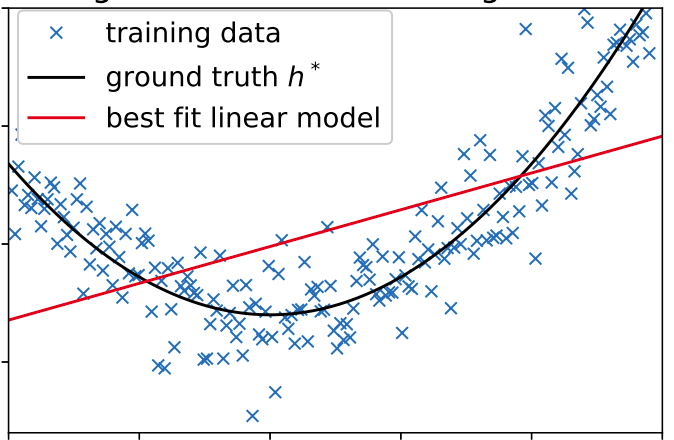
\includegraphics[width = 0.8\linewidth]{0_images/high_bias.png}
	\end{center}

	\subsection{Variance}
	When fitting a complex model, there is a large risk that we are fitting patterns in the data that happened to be present in our small, finite training set, but that do not reflect the wider pattern of the relationship between $x$ and $y$.

	“Spurious” patterns in the training
	set are (mostly) due to the observation noise, and fitting these spurious patters results in a model with large test error.

	\begin{center}
		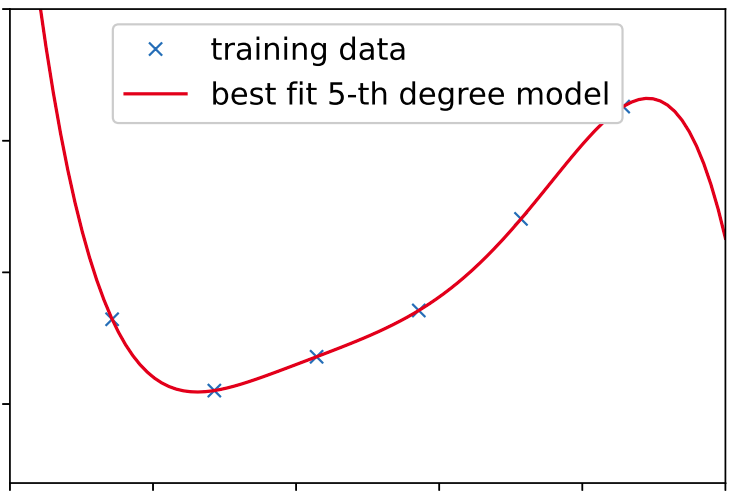
\includegraphics[width = 0.8\linewidth]{0_images/high_variance.png}
	\end{center}

	\subsection{Tradeoff}

	\begin{center}
		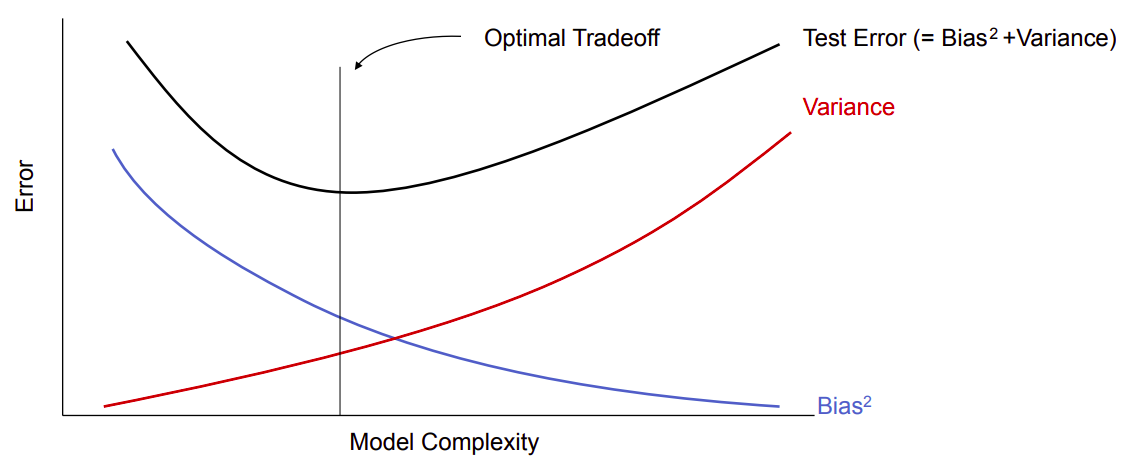
\includegraphics[width = 0.8\linewidth]{0_images/bias_variance_tradeoff.png}
	\end{center}
	\begin{itemize}
		\item More Training samples: Bias ?, Variance $\downarrow$
		\item Less Training samples: Bias ?, Variance $\uparrow^\star$
		\item Smaller set of features: Bias $\uparrow$, Variance $\downarrow$
		\item Larger Set of features: Bias $\downarrow$, Variance $\uparrow$
		\item Try email header features: Bias $\downarrow$, Variance $\uparrow$
		\item Replace the value of your last feature by a random number: Bias $\uparrow^{\star\star}$, Variance $\uparrow$
		\item Stopping Optimization early: Bias $\uparrow$, Variance $\downarrow$
	\end{itemize}
	$\star$:\textit{A specific classifier (with a fixed model complexity) will be more likely to overfit to noise in the training
		data when there is less training data, and is therefore more likely to overfit.}

	$\star\star$: \textit{Bias should increase as you are replacing information that could be useful for your
		prediction with a meaningless feature.}

	\section{Kernels}

	\textbf{Kernelizing:}

	\begin{align*}
		\text{step 1: } c^{[i](t+1)}  & = \arg\min_j \lVert x^{(t)} - \mu_j \rVert^2                                     \\
		\text{step 2: } \mu_j^{(t+1)} & = \frac{\sum_{i=1}^m 1\{c^{(t+1)} = j\}x^{(i)}}{\sum_{i=1}^m 1\{c^{(t+1)} = j\}}
	\end{align*}


	\textbf{Answer:}

	Given the formula for $c^{(t+1)}$, we want to express the distance in the feature space:

	\begin{align*}
		c^{[i](t+1)} & = \arg\min_j \lVert \phi(x^{(i)}) - \mu_j \rVert^2 \\
		             & \text{(def. of distance in feature space)}
	\end{align*}

	Expanding the squared norm, we get:

	\begin{align*}
		 & = \arg\min_j \langle \phi(x^{(i)}), \phi(x^{(i)}) \rangle + \langle \mu_j, \mu_j \rangle - 2\langle \phi(x^{(i)}), \mu_j \rangle \\
	\end{align*}

	Using the definition of the mean $\mu_j$ and the given update rules, we can expand:

	\begin{align*}
		 & = \arg\min_j \langle \phi(x^{(i)}), \phi(x^{(i)}) \rangle                        \\
		 & - 2\phi(x^{(i)})^T \left( \frac{1}{|S_j|} \sum_{l \in S_j} \phi(x^{(l)}) \right) \\
		 & \quad \text{(where $S_j = \{ l : c^{(l)} = j \}$)}
	\end{align*}

	Now, to simplify calculations in the feature space, we use a kernel function, $K(u,v) = \langle \phi(u), \phi(v) \rangle$.

	\begin{align*}
		 & = \arg\min_j K(x^{(i)}, x^{(i)})                                       \\
		 & - 2\left( \frac{1}{|S_j|} \sum_{l \in S_j} K(x^{(t)}, x^{(l)}) \right) \\
		 & + \frac{1}{|S_j|^2} \sum_{l,p \in S_j} K(x^{(l)}, x^{(p)})
	\end{align*}

	This provides a kernelized version of the update formula for $c^{(t+1)}$, where operations are defined in terms of the kernel function $K$, which implicitly computes inner products in the infinite-dimensional feature space.


\end{multicols*}
\end{document}
